
% titlepage-demo.tex
\documentclass{beamer}
\usetheme{Boadilla}
\usepackage{multirow}
\usepackage[absolute,overlay]{textpos} 
\newenvironment{reference}[2]{% 
  \begin{textblock*}{\textwidth}(#1,#2) 
      \footnotesize\it\bgroup\color{red!50!black}}{\egroup\end{textblock*}} 

\begin{document}

\begin{frame}[t]{How to Detect Event in Video?}
	\begin{itemize}
		\item State-of-the-art systems [Jiang-TRECVID2010], [Natarajan-TRECVID2011] (\textbf{best systems} in TRECVID MED 2010 and 2011)
	\end{itemize}
	
	\begin{center}
		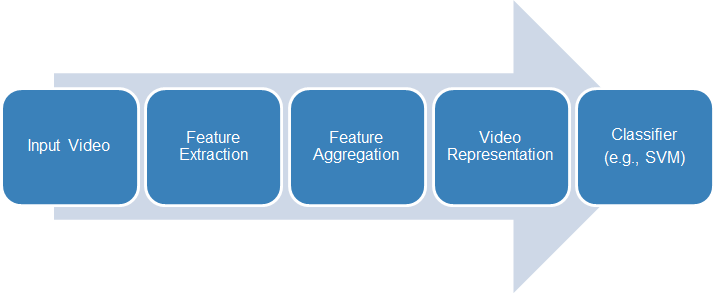
\includegraphics[width=10cm,height=4cm]{images/part2/standardapproach.png}
	\end{center}
	
	\textbf{Problem}: Neutralize the contribution of each part of the whole video. 
	\begin{itemize}
		\item In fact, the clues to determine an event often appear in a small segment.
	\end{itemize}
	
\end{frame}

\begin{frame}[t]{How to Detect Event in Small Segments of Video?}
		\begin{itemize}
\item Straightforward solutions: Split the videos into segments and detect event in these small segments. 
	\begin{itemize}
		\item $[$Niebles-ECCV2010] and [Gaidon-CVPR2011] model activities as sequences of atomic actions using semantic attributes.
		\item $[$Tang-CVPR2012] model the key segments and segment duration as latent variables and solve using a variant of HMM.
		\item $[$Vahdat-ICCV2013] Localize the most salient evidences using latent SVM. 
		\item $[$Lai-CVPR2014] Detect key instances in video based on a variant of Multiple Instance Learning. 
	\end{itemize}

\item Limitations
	\begin{itemize}
		\item Segmentation of activities into predefined atomic
		actions and annotation of these atomic actions are available.
		\item Video sequences are precisely cropped with activities of interest.
		\item Use fixed length segment. 
	\end{itemize}
			\end{itemize}
	$\rightarrow$ \textbf{We do not know what is the optimal segment length when splitting the whole video!}
	
\end{frame}

%\begin{frame}[t]{Video-based Approach}
%\begin{itemize}
%\item Features are computed over the whole video
%\item One representation for each video
%\end{itemize}

%\begin{center}
%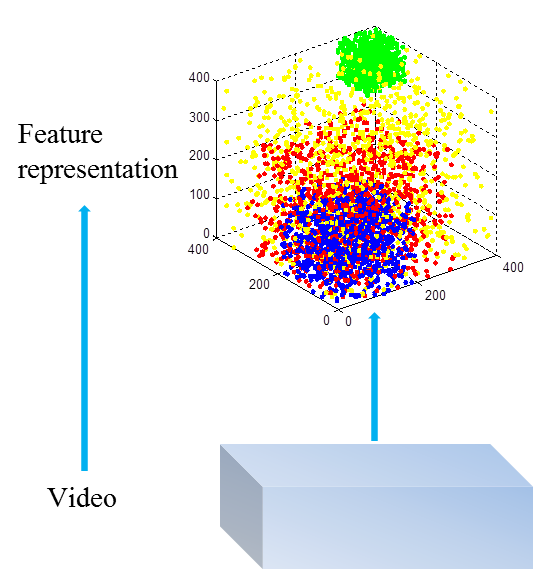
\includegraphics[width=5cm,height=4.5cm]{images/video_based.png}
%\end{center}

%\begin{itemize}
%\item Used by best MED'10 system (Columbia University)
%\item Used by best MED'11 system (BBN VISER)
%\end{itemize}

%\textbf{Specific problem}: The clues to determine an event can reside within a small segment.
%\end{frame}

\begin{frame}{Our Segment-based Approach} 
\begin{itemize}
	\item We investigate different strategies to split the videos in segments.
	\item We study the optimal segment length.
\end{itemize}
%\bigskip
\begin{columns}
  \begin{column}{0.3\textwidth}
    \centerline{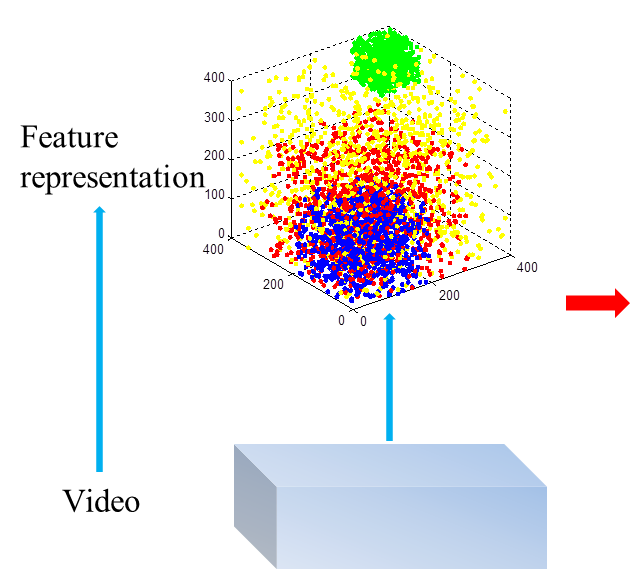
\includegraphics[width=1\textwidth]{images/video_based2.png}}
    (a) The video-based approach
  \end{column}

  \begin{column}{0.7\textwidth}
    \centerline{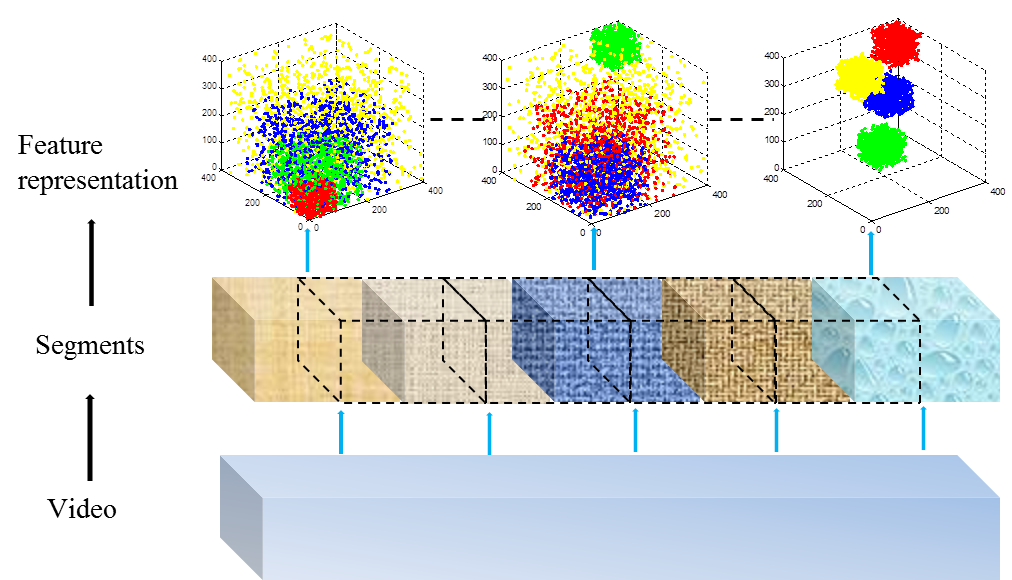
\includegraphics[width=1\textwidth]{images/segment_based.png}}
    (b) \textbf{Our proposed segment-based approach}
  \end{column}
\end{columns}
\bigskip
 
  
\end{frame}

\begin{frame}[t]{Our Segment-based Approach}
\textbf{How to select the segment length?}
\begin{itemize}
\item Non-overlapping
\begin{itemize}
	\item Uniform sampling
	\item Segment length: 30, 60, 90, 120, 200, 400 seconds 
	\item Compare with the video-based approach (using the whole video)
\end{itemize}
\item Overlapping sampling
	\begin{itemize}
	\item Uniform sampling, 50\% overlapping
	\item Segment length: 30, 60, 90, 120, 200, 400 seconds 
	\item Compare with the video-based approach (using the whole video)
	\end{itemize}
\item Segment sampling based on shot boundary detection
	\begin{itemize}
	\item Take into account the boundary information of each segment
	\item Employ the technique proposed by [Guimaraes et al. - 2003]
	\end{itemize}
	
\begin{reference}{4mm}{85mm}
Guimaraes, S.J.F., Couprie, M., Araujo, A.d.A., Leite, N.J: Video segmentation based on 2d image analysis. Pattern Recognition Letters, 2003, 24(7), 947–957.
\end{reference} 
	
\end{itemize}

\end{frame}

\begin{frame}[t]{Evaluation Framework}
\begin{center}
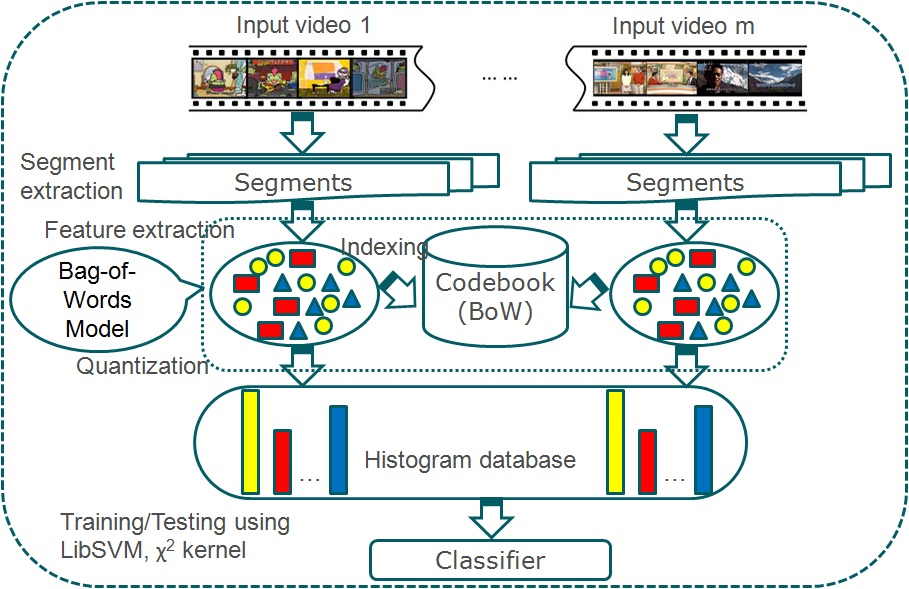
\includegraphics[width=10cm,height=6cm]{images/framework2.jpg}
\\
Evaluation framework for our event detection system.
\end{center}

\end{frame}

\begin{frame}{Experimental Setup} 	
	\begin{itemize}
		\item Dataset
		
		\begin{table}[h]
			\tiny
			\begin{tabular}{@{}|l|c|c|c|c|c|@{}}
				\toprule
				\multicolumn{1}{|c|}{Dataset} & No. Event & No. Train Videos & No. Test Videos & Total Videos & Total Hours \\ \midrule
				MED2010 & 3 & 1,744 & 1,724 & 3,468 & 110 hours \\ \midrule
				MED2011 & 10 & 12,590 & 31,822 & 33,153 & 1,400 hours \\ \midrule
				\light{MED2012} & \light{25} & \light{3,878} & \light{1,938} & \light{5,816} & \light{250 hours} \\ \bottomrule
			\end{tabular}
		\end{table}
		
		\item Feature: Dense Trajectories, MBH descriptor [Wang-CVPR2011] 	
		\item Feature encoding: Bag-of-words model, 4000 codewords.
		\item Learning: ${\chi}^{2}$ SVM.
	\end{itemize}
	
\end{frame}	

\begin{frame}{Result: Non-Overlapping vs. Overlapping Sampling} 

\bigskip

\begin{columns}
  \begin{column}{0.5\textwidth}
    \centerline{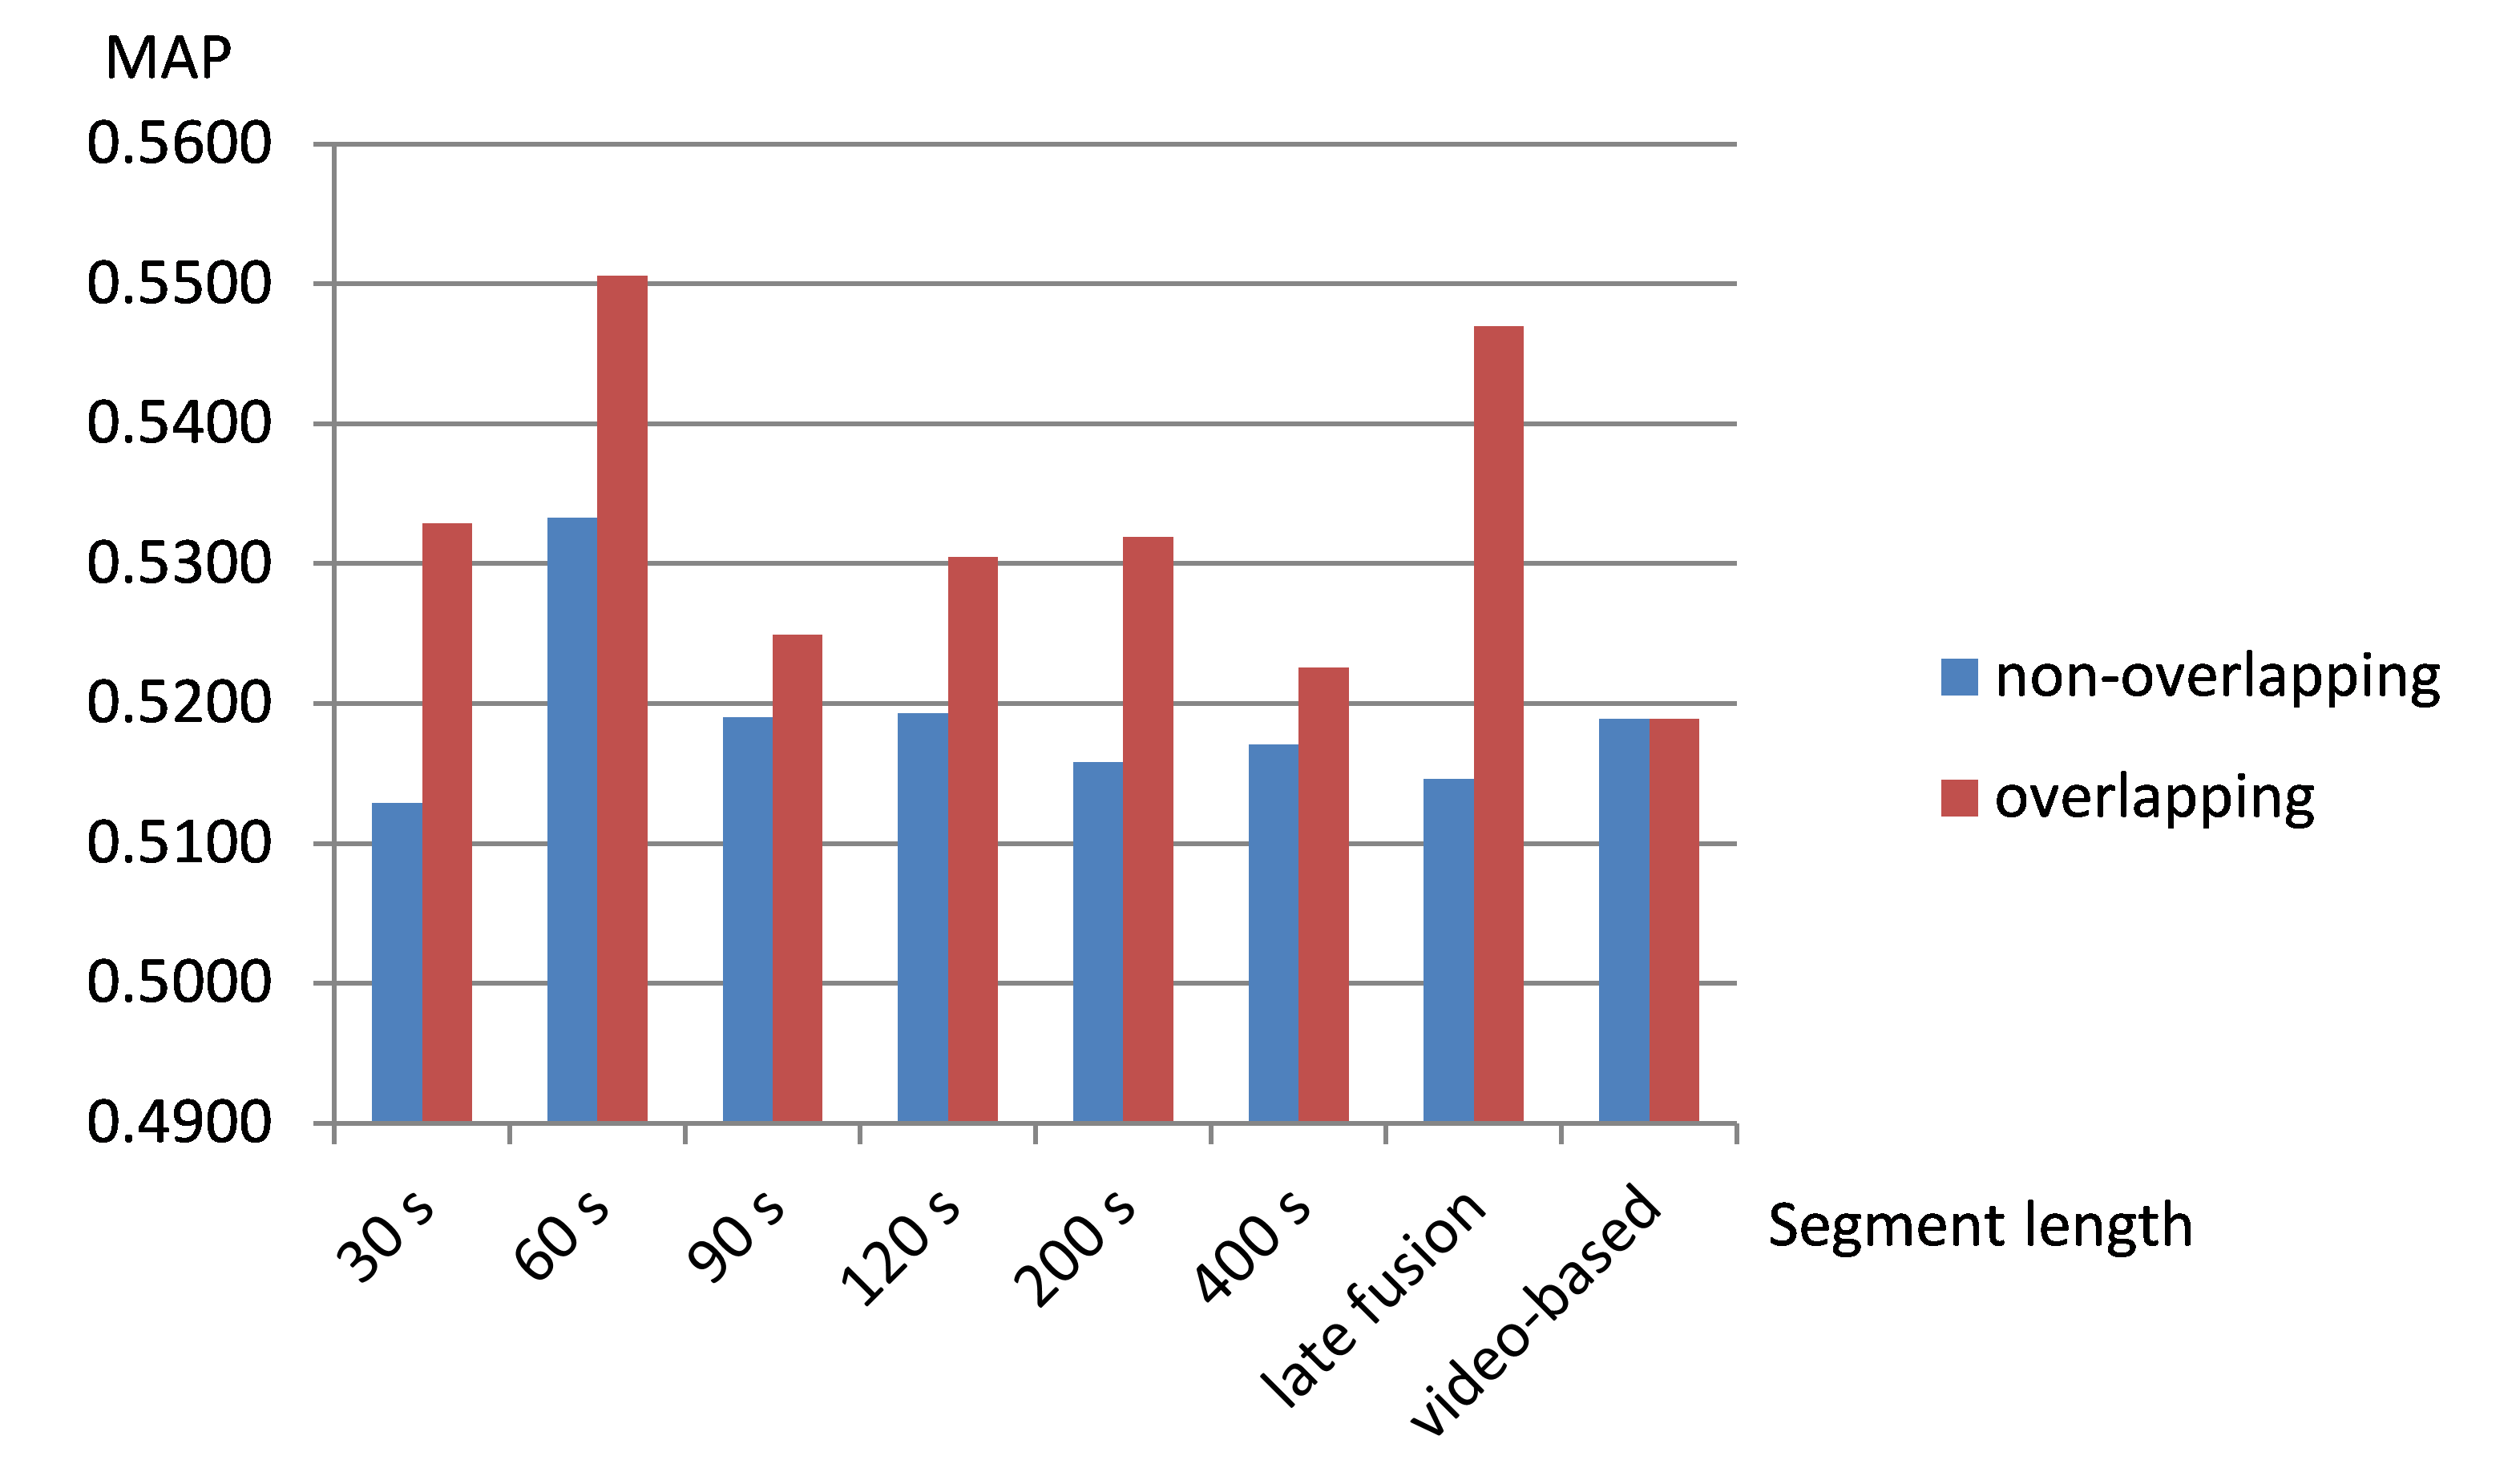
\includegraphics[width=1\textwidth]{images/med10_result.png}}
    (b) On the MED 2010 dataset
  \end{column}

  \begin{column}{0.5\textwidth}
    \centerline{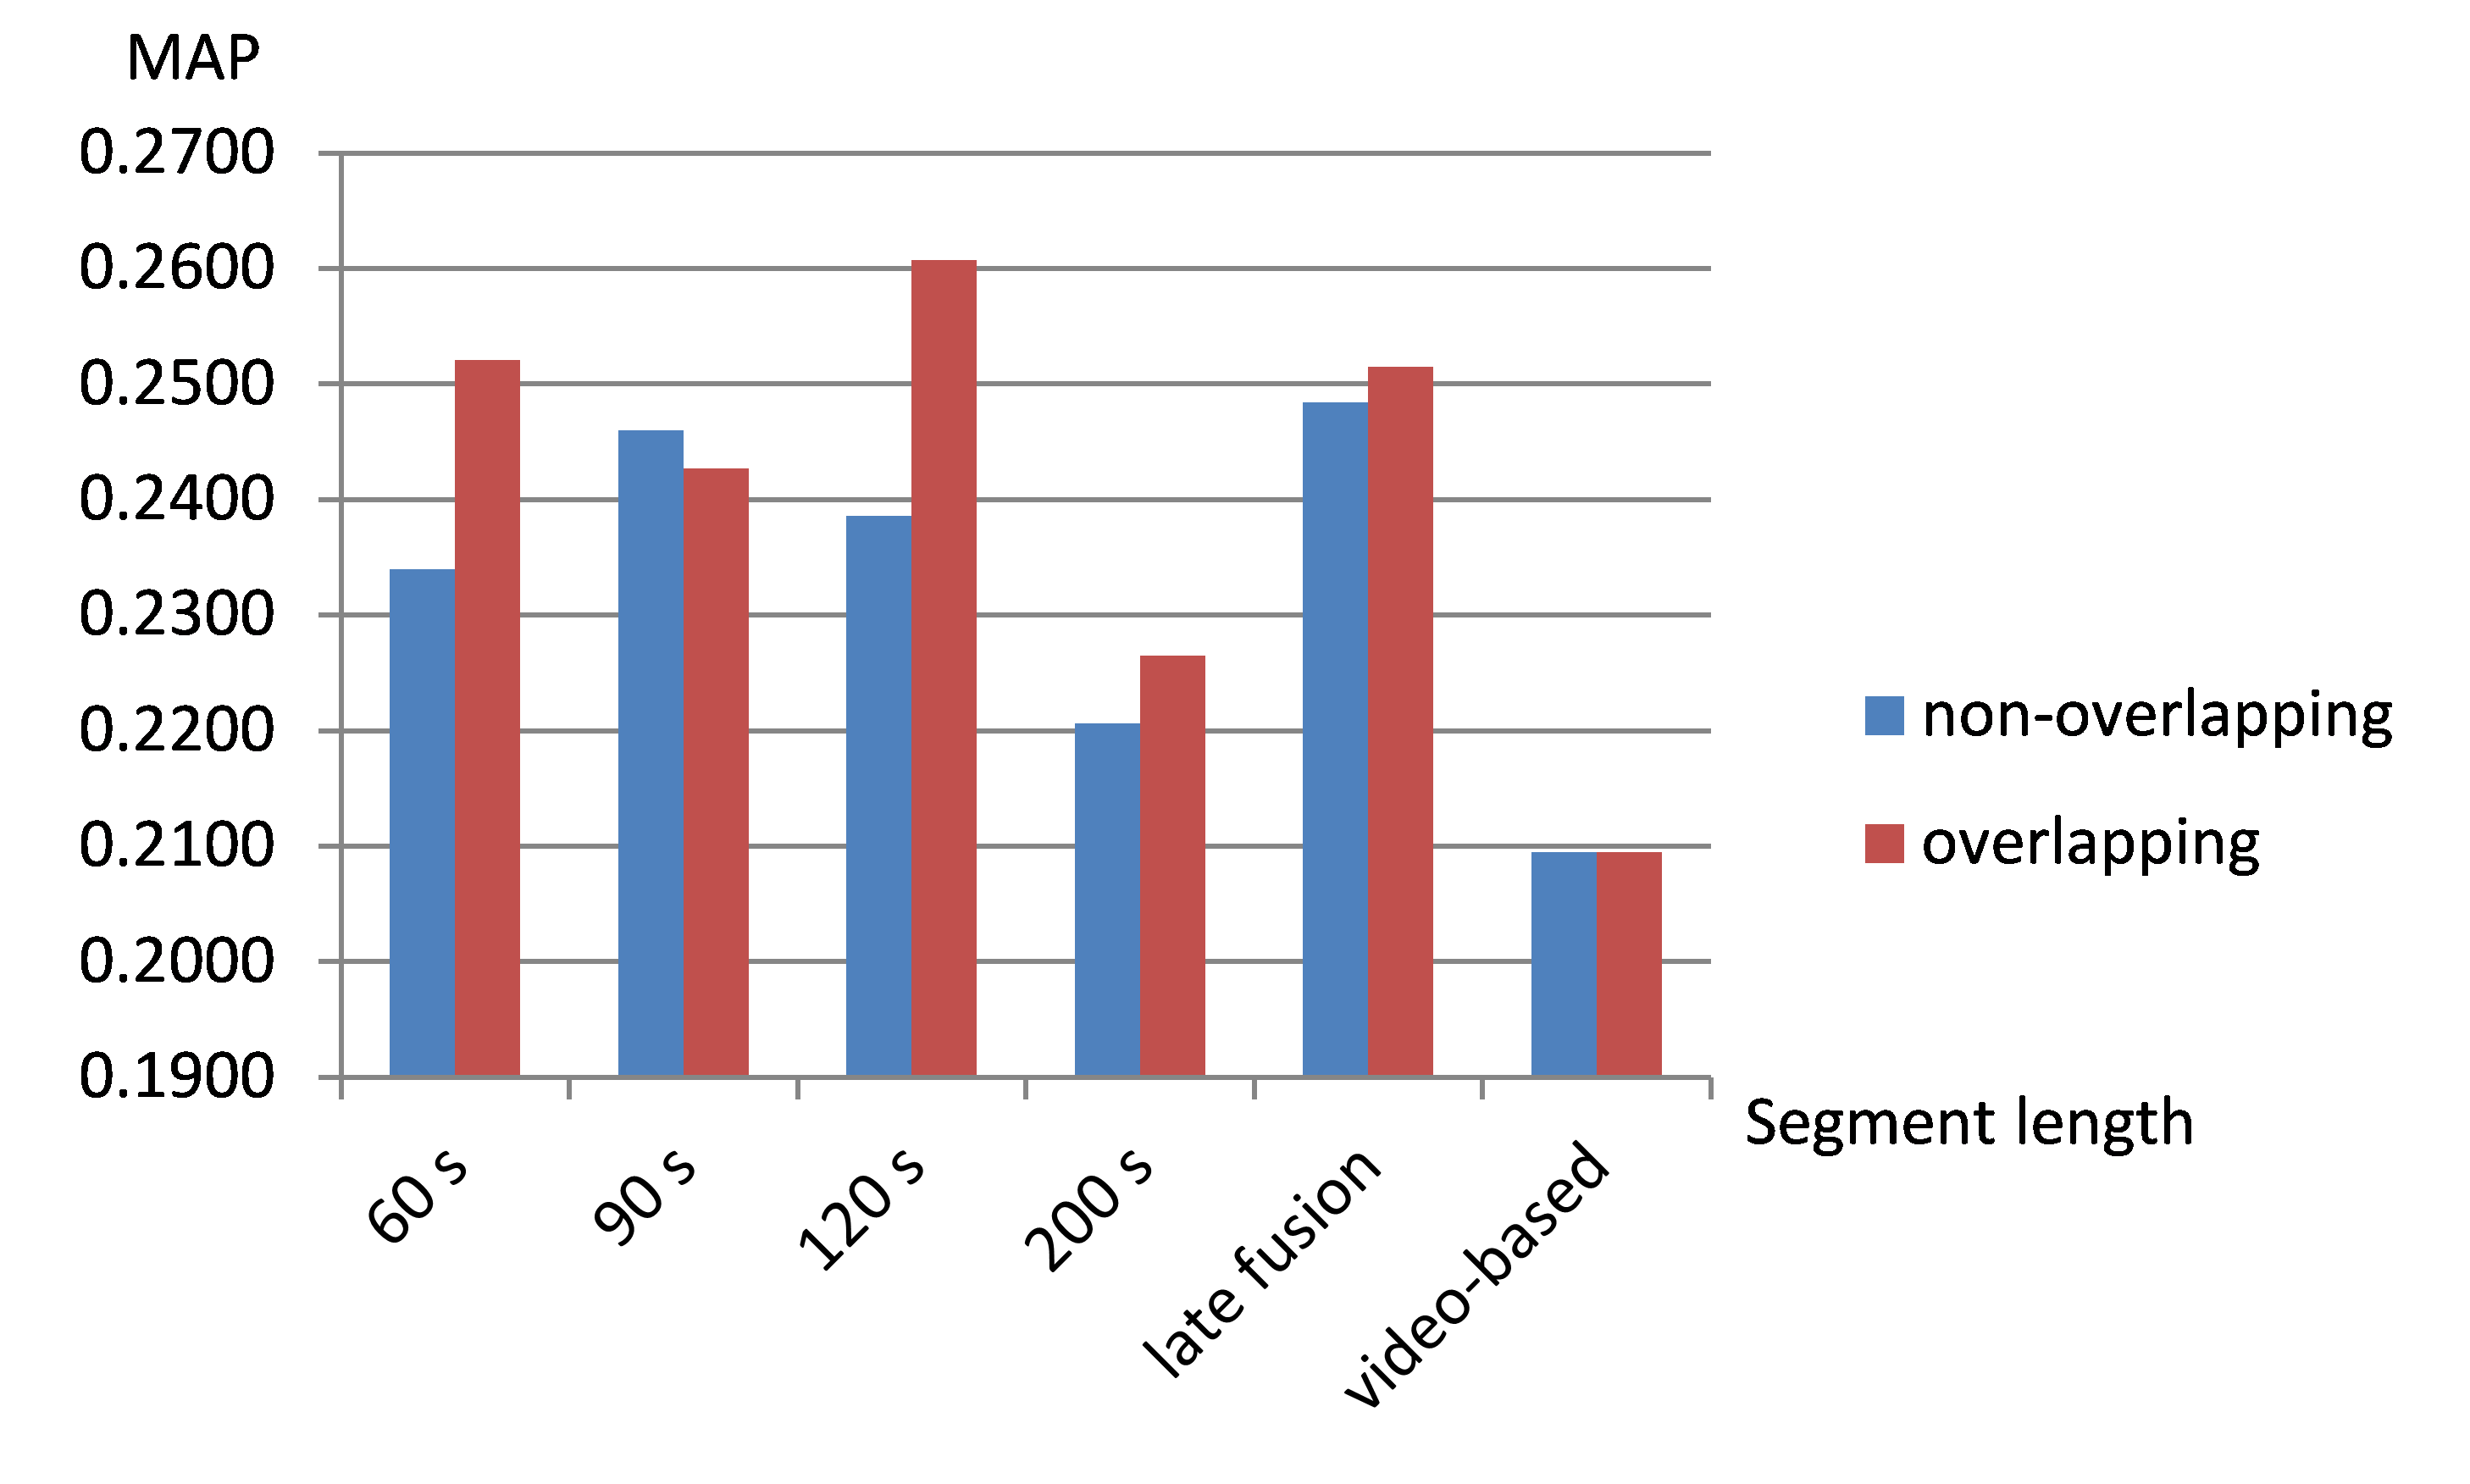
\includegraphics[width=1\textwidth]{images/med11_result.png}}
    (b) On the MED 2011 dataset
  \end{column}
\end{columns}
\bigskip

\begin{itemize}
	\item Segment-based approach significantly outperforms the Video BoW baseline.
	\item In most cases, the overlapping sampling performs the best.
\end{itemize} 

  
\end{frame}

\begin{frame}[t]{Experimental Results: On the MED 2010}
Comparison of different segment-based approaches with the video-based approach on the MED 2010 dataset.
\begin{table}
\renewcommand{\arraystretch}{1.2}
\footnotesize
\centering
% For LaTeX tables use
\begin{tabular}{| p{1.9cm} | p{1.9cm} | p{1.9cm} | p{1.9cm} | p{1.9cm} |}
\toprule
Event/MAP & Best non-overlapping & Best overlapping & SBD segments & Video-based\\
\midrule
Assembling shelter & 0.4511 & 0.4781& 0.4284  & \textbf{0.4911} \\
\midrule
Batting in a run & 0.7852 &\textbf{0.7918}& 0.7866 & 0.7902 \\
\midrule
Making a cake & 0.3636 & \textbf{0.3819} & 0.1918 & 0.2755 \\ 
\midrule
All & 0.5333 & \textbf{0.5506} & 0.4689 & 0.5189 \\
\bottomrule
\end{tabular}
\end{table}

\begin{itemize}
\item Segment-based approach outperforms the video-based approach.
\item Shot boundary detection does not work.
\begin{itemize}
	\item It is difficult to detect shot boundary with high accuracy in real videos.
\end{itemize} 
\end{itemize}

\end{frame}

\begin{frame}[t]{Experimental Results: On the MED 2011}
	\small{Comparison of different segment-based approaches with the video-based approach.}
\begin{table}
	\tiny
	\renewcommand{\arraystretch}{1}
	\label{t_med11_comparison}
	\centering
	\begin{tabular}{|c|c|c|c|c|c|c|c|}
		\hline
		\multirow{3}[4]{*}{Event} & \multicolumn{3}{|c|}{Non-overlapping sampling} & \multicolumn{3}{|c|}{Overlapping sampling} & \multirow{3}[4]{*}{Video-based} \\ 
		\cline{2-7}
		& \begin{tabular}[x]{@{}c@{}}Best\\(at 90 s) \end{tabular}
		& \begin{tabular}[x]{@{}c@{}}Late fusion\\(all lengths) \end{tabular}
		& \begin{tabular}[x]{@{}c@{}}Late fusion\\(60, 90, 120 s) \end{tabular}
		& \begin{tabular}[x]{@{}c@{}}Best\\(at 120 s) \end{tabular}
		& \begin{tabular}[x]{@{}c@{}}Late fusion\\(all lengths) \end{tabular}
		& \begin{tabular}[x]{@{}c@{}}Late fusion\\(60, 90, 120 s) \end{tabular} &  \\ \toprule
		E006  & \multicolumn{1}{|c|}{\textbf{0.1277}} & 0.1217 & 0.1244 & 0.1151 & 0.1086 & \multicolumn{1}{|c|}{0.1083} & 0.0959 \\ \midrule
		
		E007  & \multicolumn{1}{|c|}{0.1521} & 0.1419 & \multicolumn{1}{|c|}{0.1369} & 0.1552 & 0.1610 & \multicolumn{1}{|c|}{\textbf{0.1616}} & 0.1303 \\	\midrule
		E008  & \multicolumn{1}{|c|}{0.4923} & \textbf{0.4975} & \multicolumn{1}{|c|}{0.4973} & 0.4969 & 0.4903 & \multicolumn{1}{|c|}{0.4871} & 0.4766 \\	\midrule
		E009  & \multicolumn{1}{|c|}{0.2072} & 0.2145 & \multicolumn{1}{|c|}{0.2064} & \textbf{0.2160} & 0.1954 & \multicolumn{1}{|c|}{0.1958} & 0.0943 \\	\midrule
		E010  & \multicolumn{1}{|c|}{0.0916} & 0.0771 & \multicolumn{1}{|c|}{0.0753} & 0.1008 & 0.1108 & \multicolumn{1}{|c|}{\textbf{0.1109}} & 0.1020 \\	\midrule
		E011  & \multicolumn{1}{|c|}{0.0698} & 0.0805 & \multicolumn{1}{|c|}{0.0813} & \textbf{0.1591} & 0.0819 & \multicolumn{1}{|c|}{0.0845} & 0.0609 \\	\midrule
		E012  & \multicolumn{1}{|c|}{\textbf{0.3560}} & 0.3309 & \multicolumn{1}{|c|}{0.3277} & 0.3150 & 0.3293 & \multicolumn{1}{|c|}{0.3341} & 0.2858 \\	\midrule
		E013  & \multicolumn{1}{|c|}{0.6030} & 0.6033 & \multicolumn{1}{|c|}{0.6096} & \textbf{0.6188} & 0.5872 & \multicolumn{1}{|c|}{0.5910} & 0.5385 \\	\midrule
		E014  & \multicolumn{1}{|c|}{0.2008} & 0.2585 & \multicolumn{1}{|c|}{0.2579} & \textbf{0.2744} & 0.2706 & \multicolumn{1}{|c|}{0.2694} & 0.2138 \\	\midrule
		E015  & \multicolumn{1}{|c|}{0.1599} & 0.1583 & \multicolumn{1}{|c|}{0.1622} & 0.1562 & 0.1795 & \multicolumn{1}{|c|}{\textbf{0.1795}} & 0.0964 \\ 	\midrule
		All   & \multicolumn{1}{|c|}{0.2460} & 0.2484 & \multicolumn{1}{|c|}{0.2479} & \textbf{0.2607} & 0.2515 & \multicolumn{1}{|c|}{0.2522} & 0.2095 \\	\bottomrule
	\end{tabular}%
\end{table}
\begin{itemize}
	\item Segment-based approach outperforms the video-based approach.
	\item \textbf{Optimal segment length}: approximate the \textbf{mean video length}. 
	\begin{itemize}
		\item Late fusion of several runs around the mean video length.
	\end{itemize}	
\end{itemize}	

\end{frame}

\begin{frame}[t]{Conclusions}

	\begin{enumerate}
		\item \textbf{\small{Segment-based Representation (SB)}}
		\begin{itemize}
			\item Investigate different strategies to \\
			decompose a video into segments.
			\item Study the optimal segment length.
			
		\end{itemize}
			\item \light{Sum-Max Video Aggregation (SM)}
			\item \light{Event-driven Multiple Instance \\
			Learning (EDMIL)}
			
	\end{enumerate}
	
	\begin{tikzpicture}[remember picture,overlay]  
	\node [xshift=-3cm,yshift=-4.5cm] at (current page.north east)
	{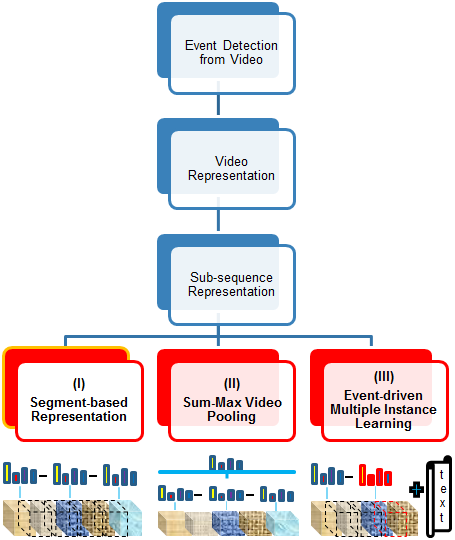
\includegraphics[width=5cm,height=7.5cm]{images/part1/contribution2.png}};
	\end{tikzpicture}
	
\end{frame}

\end{document}